\chapter{Introducción}
\label{cap:introduccion}

\begin{chapterquote}[0.87\linewidth]
El que mucho abarca poco aprieta.\\
La confianza mata al gato.\\
Más vale pájaro en mano que cien volando.\\
\smallskip
\textit{Dichos populares argentinos~\cite{chaco}}\\

\end{chapterquote}

\noindent
Suele suceder que cuando un profesional se pasa unos cuantos años trabajando en un cierto problema, comienza a dar por sentadas muchas de situaciones que el resto de las personas no tiene por qué siquiera sospechar. Personalmente, esto me ha pasado no una sino varias veces a lo largo de mi vida. Es en este sentido que esta introducción enmarca el trabajo de esta tesis académica de doctorado, indicando las diferentes fuentes de las que abrevó mi motivación a trabajar en el tema propuesto. Para ello, en lugar de elegir una dirección clara entre lo general y lo particular, iremos pasando revista a ciertos temas que contribuyeron a definir el marco este trabajo ---todos influidos por mi perfil profesional, mis convicciones personales y por supuesto, un poco de azar--- para poder justificar en la sección~\ref{sec:problemdesc} por qué el problema que queremos resolver es interesante y finalmente indicar explícitamente en la sección~\ref{sec:thesolution} cuáles son las contribuciones de este trabajo académico de doctorado.

\section{Historia de dos reactores} % TBD

Atucha~I y II
\lipsum[1]

\paragraph{Neutrones contantes y sonantes}
El martes 3 de junio de 2014 a las 9:03 el núcleo\footnote{En el sentido del inglés \emph{core}.} de la Central Nuclear Atucha~II logró mantener por primera vez una reacción nuclear de fisión en cadena autosostenida. Este suceso marcó un hito no sólo en la industria nuclear argentina sino también en mi carrera profesional. Durante cinco años y medio estuve trabajando desde TECNA S.A. junto a un equipo ingenieros de Nucleoeléctrica Argentina~S.A. en el desarrollo de modelos y códigos de cálculo acoplados para predecir, estudiar y analizar el comportamiento de la central teniendo en cuenta neutrónica espacial, realimentaciones termohidráulicas y acciones del sistema de control, limitación y protección del reactor (en el apéndice~\ref{ap:publicaciones} se puede consultar una lista de publicaciones e informes técnicos relacionados a mi trabajo en Atucha~II). Esa mañana pude presenciar de primera mano las indicaciones de los instrumentos que mostraban un incremento lineal en el tiempo de la señal de nivel de flujo neutrónico en el núcleo del reactor, que es lo que yo había leido en los libros de texto que debía suceder en un reactor crítico en presencia de una fuente independiente de neutrones. Para terminar de despejar cualquier clase de dudas (incluyendo físicas, tecnológicas e industriales), durante los siguientes meses continué dando soporte de ingeniería a las tareas de aumento escalonado de potencia hasta el cien por ciento, obteniendo evidencia experimental a prueba de escépticos de que realmente el reactor era capaz de generar potencia térmica a partir de la fisión del uranio mediante reacciones inducidas por neutrones.

\paragraph{Más de una rueda de auxilio}
Aún cuando no son deseados, los imprevistos existen. Es por eso todos nos aseguramos de que la rueda de auxilio de nuestro auto esté en condiciones ante de emprender un viaje más o menos largo ya que existe una probabilidad~$p_1$ no nula de que se nos pinche una cubierta en el camino.  ¿Pero por qué decimos \emph{la} rueda de auxilio y no \emph{las} ruedas de auxilio? ¿Acaso la probabilidad~$p_2 \approx p_1^2$ de pinchar no una sino \emph{dos} cubiertas no es también diferente de cero al fin y al cabo? Sí, pero esa probabilidad~$p_2$ es tan pequeña que no vale la pena el esfuerzo y el costo que implica llevar dos ruedas de auxilio en nuestro automóvil. Llegado el caso, llamamos a la grúa. En el diseño de centrales nucleares usamos un razonamiento similar: para todos los eventos cuyas probabilidades~$p_i$ de ocurrencia sea significativas (accidentes de base de diseño) debemos tomar precauciones; para el resto (accidentes fuera de la base de diseño), preparamos soluciones de contingencia.

En general, los reactores nucleares de potencia necesitan más de un único mecanismo de extinción de las reacciones de fisión. El primero son las mismas barras de control, que son insertadas rápidamente dentro del núcleo para absorber neutrones y no permitir que las fisiones se autosostengan en el tiempo. Si bien la probabilidad de que este mecanismo falle es pequeña en términos absolutos, debemos incluir al menos un sistema más de extinción del reactor redundante, diverso e independiente. En el caso de las Centrales Nucleares tipo Atucha, el segundo sistema de extinción del reactor consiste en inyectar rápidamente una solución de ácido deuterobórico en el tanque del moderador. De esta forma, como los núcleos\footnote{En el sentido del inglés \emph{nuclei}.} de $^{10}$Bo son grandes absorbentes de neutrones, las reacciones de fisión se extinguen a medida que el boro ingresa a la zona del núcleo del reactor.

\paragraph{La conexión europea}
Fue condición necesaria para la puesta a crítico de la central, la preparación del Informe Final de Seguridad y su presentación a la Autoridad Regulatoria Nuclear. Si bien la mayor parte de la ingeniería necesaria para su elaboración fue realizada en el país, debido a ciertas características del proyecto Atucha~II, para la evaluación de algunos aspectos relacionados al Capítulo~15 de Análisis de Accidentes fueron contratados consultores del exterior. En particular, el modelado de la actuación del sistema de inyección de boro de emergencia y su efecto sobre la neutrónica durante casos accidentales fue uno de éstos aspectos. Por un lado involucra cierto know-how y técnicas que no estaban completamente desarrolladas en el país al momento de comenzar los trabajos de licenciamento de la central. Por otro lado, suele ser una buena práctica involucrar a grupos internacionales especializados, sobretodo en temas complejos, delicados y sensibles.

\begin{figure}[p]
 \begin{center}
  \subfloat[Esquema de dos pasos estimando la primero reactividad~$\rho_b(t)$ debida a la inyección de boro y luego incorporándola a las ecuaciones de cinética puntual.]
  {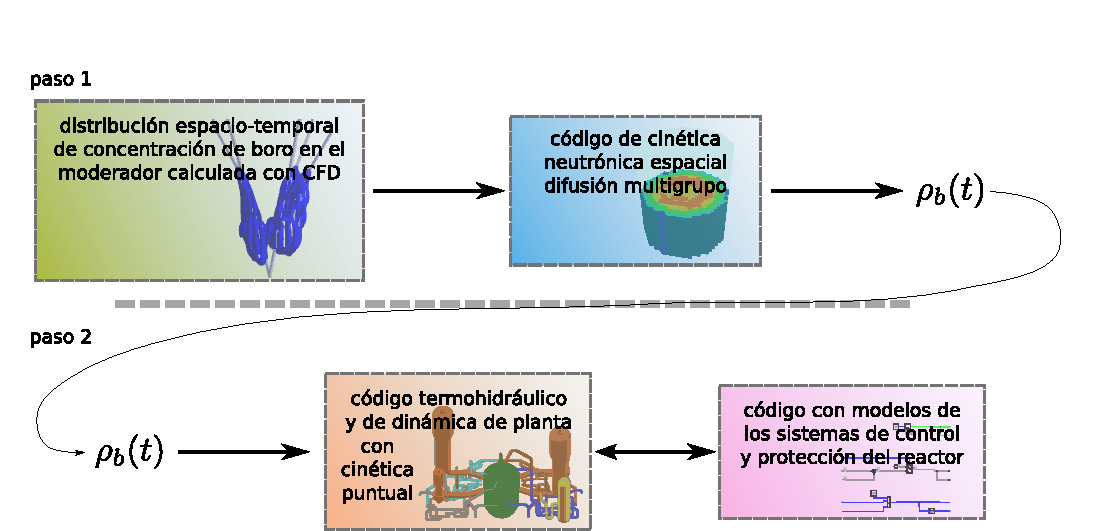
\includegraphics[scale=0.8]{introduccion/borocinetica}}

\vspace{2.5cm minus 1cm}

  \subfloat[Esquema completamente acoplado utilizando cinética neutrónica espacial.]
  {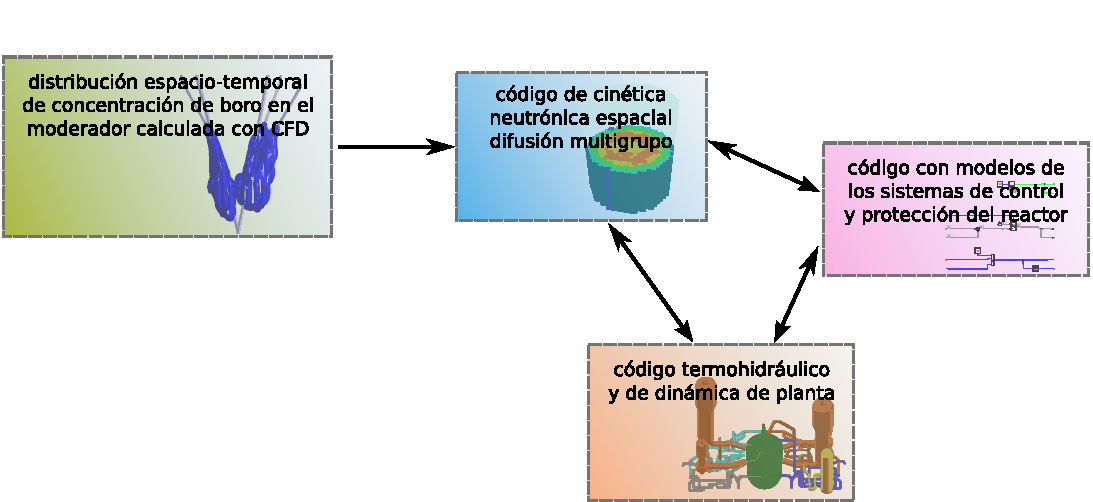
\includegraphics[scale=0.8]{introduccion/borofull3d}}
 \end{center}
\caption{\label{fig:acopleboro}Esquema de acople propuesto para el modelado de accidentes que involucran la actuación del sistema de inyección de boro de emergencia en la Central Nuclear Atucha~I. La primera alternativa es calcular la reactividad negativa debida a la inyección de boro y luego incorporar~$\rho_b(t)$ a la reactividad total de las ecuaciones de cinética puntual. La segunda consiste en un esquema completamente acoplado utilizando cinética neutrónica espacial. En cualquier caso, la forma de incorporar la distribución espacio-temporal de concentración de boro en el moderador al código neutrónico es la misma.}
\end{figure}


\paragraph{Aprendiendo de los que saben} A partir de la experiencia ganada desde la interacción con estos expertos y de las capacidades propias desarrolladas durante el proceso de licenciamento de Atucha~II, que han servido incluso para que los consultores externos mejoren tanto sus propias capacidades como los resultados provistos, es que a comienzos de 2014 Nucleoeléctrica decidió que las tareas de actualización del Informe Final de Seguridad de la Central Nuclear Atucha~I utilizando modelos, métodos y códigos según el estado del arte actual (i.e. los modelos, métodos y códigos usados para licenciar Atucha~II) sean realizadas íntegramente en el país por ingenieros argentinos. En particular, la evaluación de la reactividad negativa insertada por el sistema de inyección de emergencia y de los efectos espaciales de la interacción neutrónica-termohidráulica durante accidentes recae ahora bajo la órbita del mismo equipo de trabajo (el nuestro) que antes había contratado consultores europeos para realizar dichas 
tareas de ingeniería~\cite{ing2014-boro}. Durante 2014 hemos trabajado en el diseño un esquema de cálculo acoplado basado en recursos de memoria compartida para permitir que durante el 2015 se realicen los estudios necesarios para analizar una treintena de accidentes de base de diseño que componen el Capítulo~15 del FSAR de la Central Nuclear Atucha~I.

\begin{figure}[p]
\begin{center}
 \subfloat[\label{fig:arrayatucha}Atucha (canales verticales)]{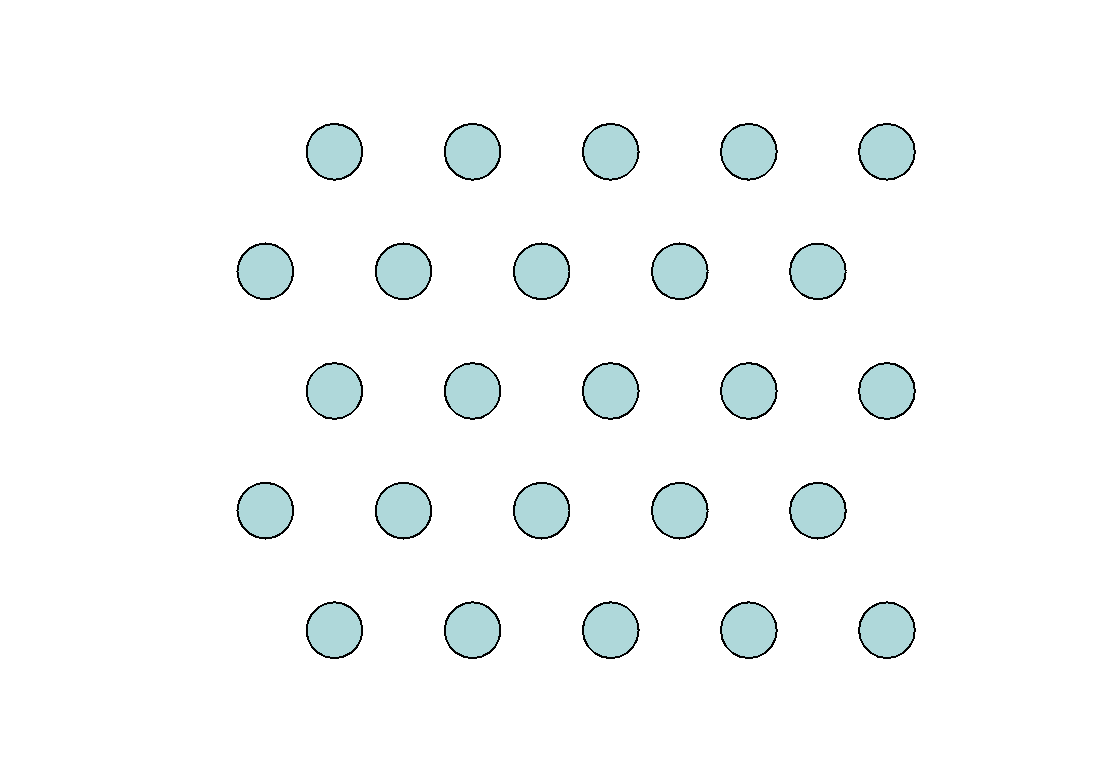
\includegraphics[scale=0.33]{array/array2d-atucha}} \hspace{2cm}
 \subfloat[\label{fig:arraycandu}CANDU (canales horizontales)]{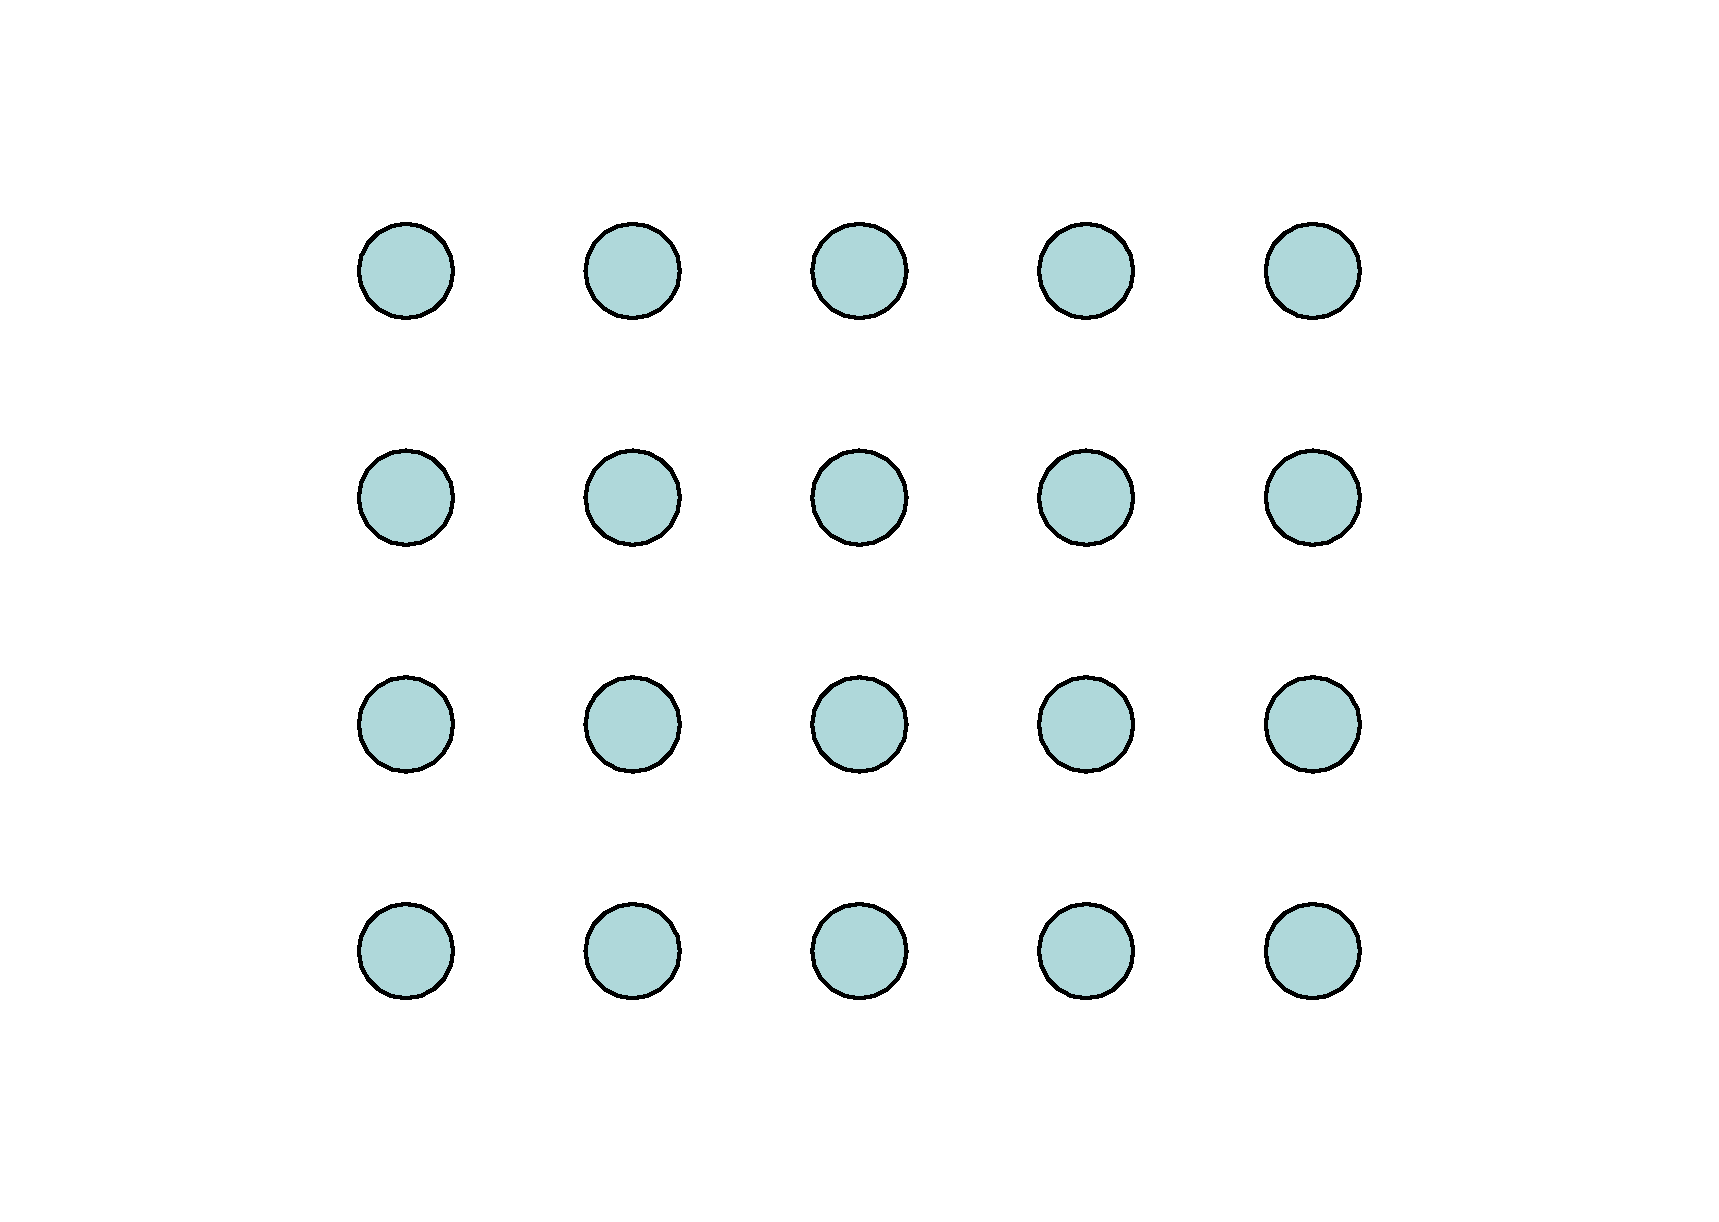
\includegraphics[scale=0.33]{array/array2d-candu}}
\end{center}
\caption{\label{fig:arrays}Arreglo de canales en el plano perpendicular a la dirección axial en los reactores de agua pesada que operan en la Argentina. En ambos casos los canales están inmersos en un tanque que contiene agua pesada que actúa como moderador de los neutrones que nacen en los elementos combustibles alojados en los canales. Ambas figuras están representadas en la misma escala espacial, por lo que se puede observar la diferencia en los pasos y en los radios de los canales.}
\end{figure}

\begin{figure}[p]
\begin{center}
\includegraphics[width=0.7\linewidth]{introduccion/celdascna1}
\end{center}
\caption{\label{fig:celdacna1} Celda neutrónica unitaria para el núcleo de Atucha~I~\cite{aatn-xs-2014}. El cálculo de celda se realiza sobre un círculo de radio equivalente a la celda hexagonal geométrica. El cálculo de núcleo utiliza las secciones eficaces homogeneizadas a dos grupos y las aplica a una celda rectangular. Esta última celda es la que define la malla de representación de la figura~\ref{fig:mallareprpce}.}
\end{figure}

\paragraph{Claro como el agua pesada}
En los reactores de agua pesada presurizada, si bien las funciones de refrigeración del combustible y moderación de los neutrones son realizadas por el mismo material (justamente agua pesada), las condiciones de temperatura a las que se encuentran refrigerante y moderador son diferentes. Incluso en ciertos diseños y/o condiciones operacionales, la presión puede ser diferente. Por lo tanto, desde el punto de vista neutrónico se deben considerar como materiales diferentes.
El núcleo consiste en un arreglo periódico de canales refrigerantes con sus ejes paralelos entre sí. En los reactores tipo Atucha los canales se encuentran en forma vertical y con un arreglo sobre el plano transversal basado en triángulos equiláteros, mientras que éstos son horizontales y distribuidos como vértices de cuadrados en reactores tipo CANDU~(figura~\ref{fig:arrays}). Los canales están inmersos en un gran tanque que contiene el moderador líquido, que usualmente se mantiene más frío que el refrigerante con el objetivo de mejorar la moderación y aumentar así el factor de multiplicación infinito~$k_\infty$ del núcleo. El elemento combustible está compuesto por un arreglo de barras individuales (37 en Atucha, 36 en CANDU) que contienen las pastillas de dióxido de uranio recubiertas por un cladding de zircaloy.

En este tipo de reactores la parada rápida del reactor se realiza mediante la inserción de las barras de control por gravedad. El segundo sistema de extinción consiste en la inyección rápida de una solución líquida absorbente de neutrones en el tanque del moderador. En particular, para el caso de Atucha~I y~II se emplea ácido deuterobórico con boro enriquecido en su isótopo diez. 

 


% exportado en 1206x852 desde paraview a 225 dpi
\begin{figure}[p]
\begin{center}
 \subfloat[\label{fig:mallareprpce}Malla de representación superpuesta a una malla de cálculo de $4 \times 4 \times 20$. La escala de colores indica el quemado de combustible por celda unitaria]{\begin{minipage}{\linewidth}\begin{center}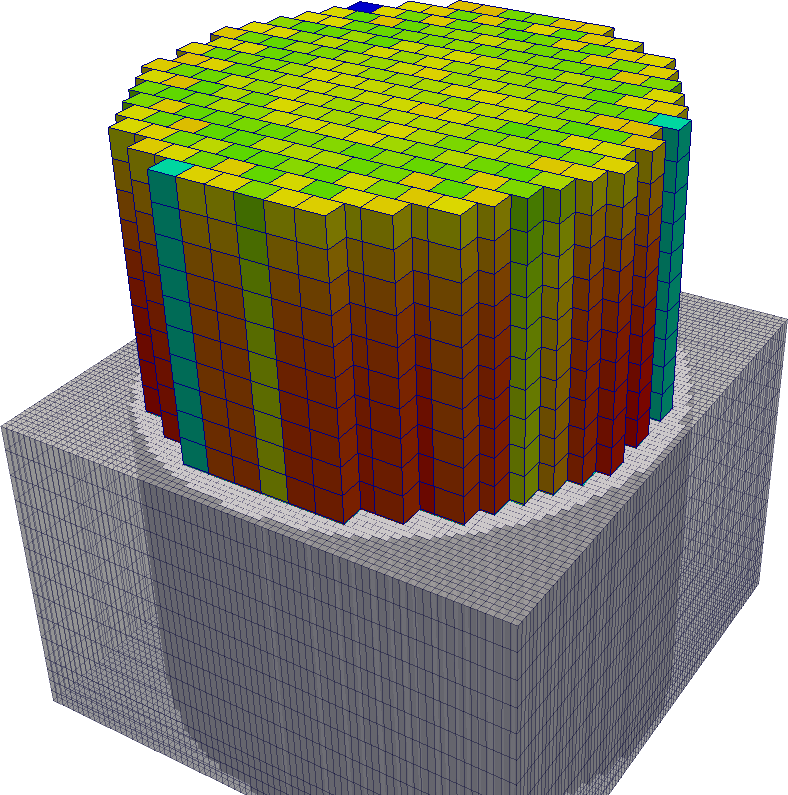
\includegraphics{introduccion/cna1rep.png}\end{center}\end{minipage}}

 \subfloat[\label{fig:mallacalcpce}Malla de cálculo de $4 \times 4 \times 20$ indicando sección eficaz total térmica. Se puede observar el efecto ``escalera'' de la discretización espacial en el tanque del moderador y de los tubos guía de las barras de control.]{\begin{minipage}{\linewidth}\begin{center}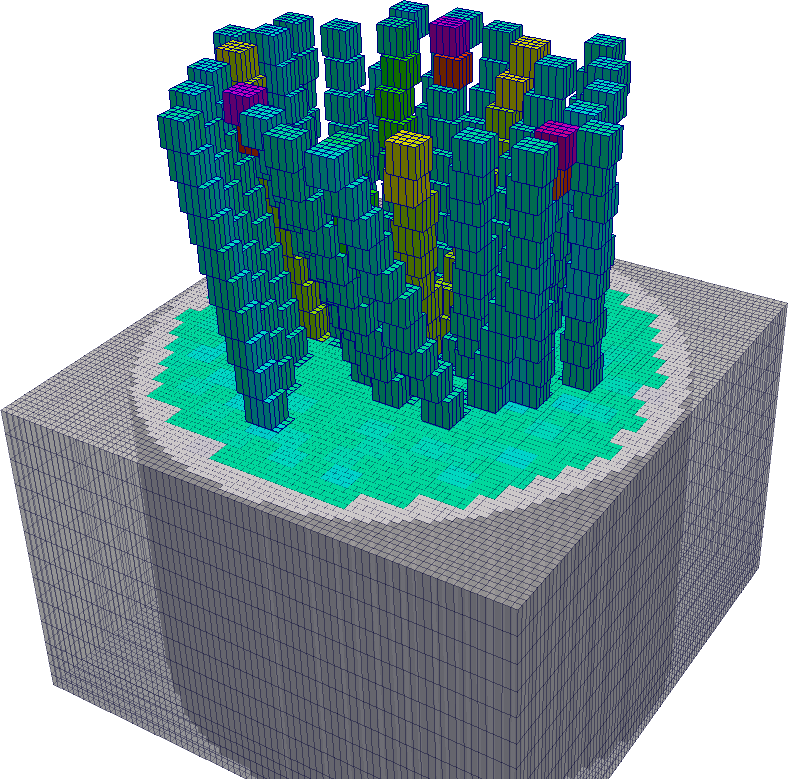
\includegraphics{introduccion/cna1calc.png}\end{center}\end{minipage}}
\end{center}
\caption{\label{fig:mallaspce} Mallas de representación y de cálculo propias del código neutrónico utilizado en el esquema acoplado propuesto de la figura~\ref{fig:acopleboro} para Atucha~I. Las figuras fueron generadas con la herramienta libre ParaView (apéndice~\ref{paraview}) a partir de extensiones al código neutrónico original realizadas por el autor del esta tesis durante sus trabajos para el licenciamento de la Central Nuclear Atucha~II~\cite{aatn-pumita-2014}.}
\end{figure}


\paragraph{Dos son compañía, tres son multitud}
Podemos estudiar la mayoría de los casos que componen el Capítulo~15 ``Análisis de accidentes'' del FSAR utilizando cinética neutrónica puntual separando las contribuciones individuales~$\rho_x(t)$ debido al efecto~$x$ (barras de control, temperaturas, densidades, xenón, etc.) y luego sumándolas algebráicamente  para obtener una reactividad total~$\rho(t)$. Sin embargo, en algunos casos tales como los accidentes con pérdida de refrigerante, es importante que consideremos efectos espaciales al presentarse una retroalimentación compleja debido tanto a las características termohidráulicas como neutrónicas de este tipo de reactores. Ambas situaciones son tenidas en cuenta en el esquema acoplado propuesto, que ilustramos en la figura~\ref{fig:acopleboro}. En él se involucra a un código de planta, a un modelo de la lógica de control y protección del reactor y a un código de cinética espacial capaz de incorporar distribuciones espacio-temporales de propiedades, en particular concentración de boro en el moderador, 
calculadas a partir de técnicas tipo Computational Fluid Dynamics. 


\paragraph{Multifísica multiescala}
En cualquiera de los dos casos ilustrados en la figura~\ref{fig:acopleboro} para la evaluación de la neutrónica asociada a la actuación del sistema de inyección de boro de emergencia, el código neutrónico resuelve la ecuación de difusión de neutrones en el núcleo con secciones eficaces macroscópicas homogeneizadas espacialmente a nivel de canal refrigerante individual y condensadas a dos grupos de energía. Es decir, la celda unitaria que se resuelve en el nivel de cálculo de celda en el esquema multi-escala usual (sección~\ref{sec:multiescala}) contiene un canal refrigerante con las barras que componen el elemento combustible y una porción de moderador asociada a dicho canal~(figura~\ref{fig:celdacna1}).

\medskip

El código de núcleo trabaja con dos mallas (o retículas según la nomenclatura propuesta por el autor original del código), ambas estructuradas: una de representación y una de cálculo (figura~\ref{fig:mallaspce}). En la primera es donde se definen las secciones eficaces macroscópicas que dependen de las propiedades medias de la celda: quemado y temperatura de combustible, temperaturas y densidades de moderador y refrigerante, concentración de boro en moderador y refrigerante, concentración de xenón~135 en el combustible, etc. En la segunda, que es una subdivisión de la primera, es donde se resuelve numéricamente la ecuación de difusión de neutrones a partir de las secciones eficaces definidas sobre la malla de representación.

Para el caso particular de Atucha~I, en la malla de representación define la ubicación espacial de los 253 canales. La malla de cálculo resulta de dividir sobre el plano $x$-$y$ el rectángulo asociado a cada celda en~$n\times n$ rectángulos más pequeños (por la geometría del arreglo de canales~$n$ debe ser una potencia de dos) y la longitud activa~$h$ del núcleo en una cantidad~$m$ de celdas axiales. En el equipo de trabajo entonces se dice que un cálculo se realiza con una malla de de $2\times 2 \times 20$, $4\times 4 \times 80$, etc. La figura~\ref{fig:mallacalcpce} muestra una malla de cálculo de $4 \times 4 \times 20$. 

\begin{figure}[b!]
 \begin{center}
  \includegraphics{introduccion/gota}
 \end{center}
\caption{\label{fig:gota}Efecto de dilución geométrica de secciones eficaces. Una pequeña gota de absorbente al ser diluida en el volumen de una celda mucho mayor utilizando sólo relaciones geométricas resulta en secciones eficaces homogeneizadas excesivamente absorbentes. Un absorbente negro del 5\% del volumen de una celda transforma la celda completa en un absorbente casi negro.}
\end{figure}

\begin{figure}[p]
 \begin{center}
\includegraphics{introduccion/cfd}
 \end{center}
\caption{\label{fig:cfd}Cálculo fluidodinámico de la evolución temporal de la pluma de boro en el tanque del moderador de Atucha~I realizada por ingenieros de NA-SA con técnicas CFD sobre una malla no estructurada de aproximadamente 4.5 millones de celdas~\cite{enief-2014-cpl}. Se pueden observar los huecos en la distribución espacial generados por la presencia de los canales.}

 \begin{center}
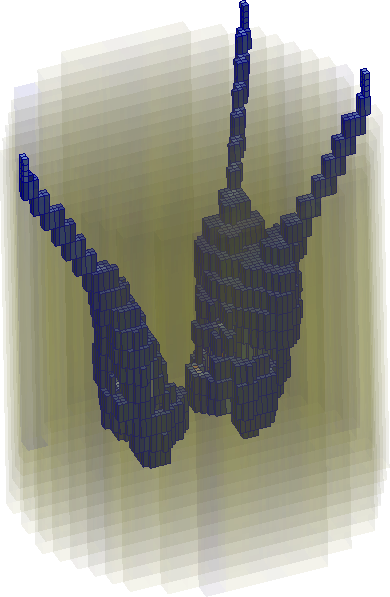
\includegraphics{introduccion/boropce}
 \end{center}
\caption{\label{fig:boropce}Mapeo de la distribución instantánea de boro a una malla de cálculo del código neutrónico de núcleo de $4 \times 4 \times 20$ ($\sim$ 200.000 celdas)~\cite{enief-2014-cpl}. No es posible observar la presencia de los canales.}
\end{figure}

\paragraph{Calcule un litro y obtenga dos (por el mismo precio)}
Durante la interacción con los consultores extranjeros en la etapa de evaluación de la inyección de boro en Atucha~II hemos identificado que una discretización espacial gruesa tiende a sobrestimar la reactividad negativa introducida de forma inaceptable debido al efecto de dilución de secciones eficaces que repasamos a continuación. En efecto, consideremos una pequeña gota de ácido deuterobórico con una gran concentración de boro, digamos 2000 partes por millón, que en algún instante se encuentra dentro de una de las celdas sobre las cuales se homogeneizan las secciones eficaces macroscópicas, como ilustramos en la figura~\ref{fig:gota}, y supongamos que la gota ocupa el 5\% del volumen de la celda. Para poder avanzar un paso del cálculo cinético-espacial de núcleo debemos asignarle secciones eficaces mascroscópicas a la celda que contiene la pequeña gota de boro, a partir de cálculos paramétricos de nivel de celda en los cuales conocemos cómo varían las secciones eficaces en función de los parámetros 
termohidráulicos (temperaturas y densidades) y de la concentración de venenos (xenón y boro) de la celda. Como el boro no está uniformemente distribuido, debemos obtener un valor medio que proponemos calculars como un promedio de las concentraciones de boro de la gota y del resto de la celda pesado con los volúmenes relativos. Para el caso de la figura~\ref{fig:gota}, la concentración media de boro de la celda sería 100 ppm, resultando en una absorción casi negra para toda la celda en lugar de una absorción completamente negra sólo en el 5\% del volumen. La alternativa a la dilución geométrica sería homogeneizar de forma tal no de mantener la relación de volúmenes sino los ritmos de reacción. Esto implicaría tener que realizar un nuevo cálculo de celda para cada una de las celdas de la malla de representación para cada instante de tiempo teniendo en cuenta la geometría real de la gota, lo que de hecho está fuera de las posibilidades de las cadenas de cálculo actuales, pero podría llegar a ser un esquema alternativo. Sin embargo, como discutimos más adelante, aún existen otros inconvenientes en la formulación que no pueden ser salvados de esta forma.


\begin{figure}[t]
 \begin{center}
\subfloat[$4 \times 4 \times 40$]{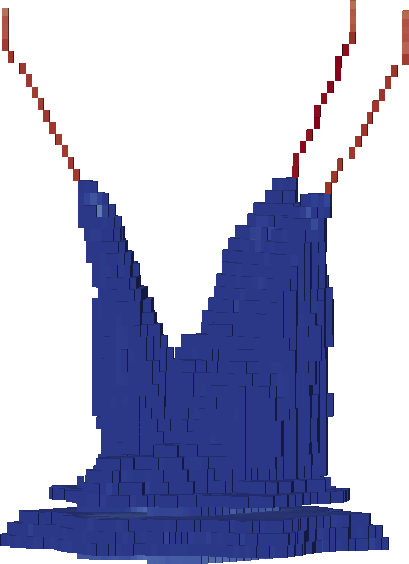
\includegraphics{introduccion/4x4-40}}\hspace{\fill}
\subfloat[$4 \times 4 \times 60$]{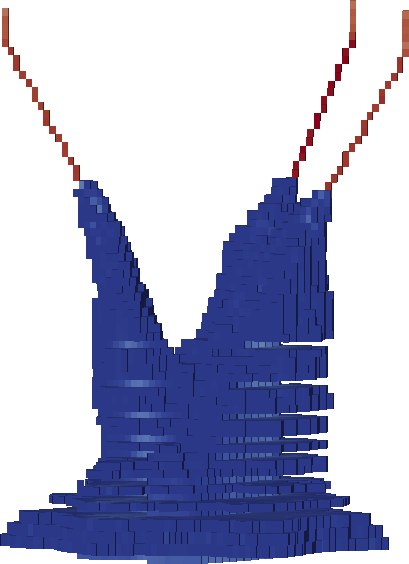
\includegraphics{introduccion/4x4-60}}
 \end{center}
\caption{\label{fig:4x4}Distribución de boro para un cierto instante mapeada desde la malla de CFD a la malla de cálculo neutrónico de $4 \times 4$ con (a) 40 celdas axiales y (b) 60 celdas axiales \cite{aatn-aet-2014}. En el segundo caso con las celdas más pequeñas, el mapeo de malla no estructurada (CFD) a malla estructurada (neutrónica) no pueda reproducir los resultados en las zonas donde la malla de CFD no está suficientemente refinada. El resultado es que en forma espuria se remueve boro del tanque del moderador para mallas de cálculo neutrónico demasiado finas.}
\end{figure}

Para reducir este efecto y además poder realizar estudio de convergencia de malla hemos decidido extender el código de núcleo para permitir que la definición de la distribución instantánea de boro pueda realizarse también sobre la malla de cálculo, en lugar de hacerlo sólo sobre la de representación como el resto de los parámetros (temperaturas, densidades, etc.)~\cite{aatn-pumita-2014}. En este caso, a partir de resultados fluidodinámicos es que incorporamos la pluma de boro al esquema de cálculo acoplado mapeando las celdas la mallas del código CFD (figura~\ref{fig:cfd}, $\sim$ 4.5 millones de celdas) a la malla de cálculo del código neutrónico (figura~\ref{fig:boropce}, $\sim$ 200.000 celdas para $4\times 4 \times 20$).




\paragraph{Celdas refinadas}
Dado que el efecto de dilución de secciones eficaces macroscópicas se reduce drásticamente con el tamaño de la celda, hemos realizado estudios de convergencia de malla~\cite{aatn-aet-2014} con el doble objetivo de estimar los errores cometidos y para extrapolar las reactividades obtenidas a una discretización espacial infinitesimal. Sin embargo, hemos encontrado que no siempre es conveniente trabajar con mallas de cálculo neutrónico demasiado finas. En la figura~\ref{fig:4x4} mostramos el resultado de mapear una cierta distribución de concentración de boro para dos mallas de cálculo similares, una con 40 celdas axiales y otra con 60. Debido a que el cálculo CFD se realiza sobre una malla no estructurada, ésta se ha diseñado de forma tal de ser más refinada en ciertas ubicaciones de interés dentro del tanque del moderador. En algunas zonas donde esta malla es más gruesa, sucede que las celdas de CFD son más grandes que las celdas de cálculo neutrónico. El resultado es que, para mallas neutrónicas demasiado 
finas, pueden quedar algunas celdas sin tener asignada una concentración de boro ya que todo el boro de la celda CFD podría asignarse a una celda neutrónica vecina. De esta manera, a partir de un cierto tamaño de malla neutrónica, si bien se disminuye el efecto de la dilución de secciones eficaces sucede que en forma numérica se remueve boro del tanque del moderador. Estos dos efectos tienen consecuencias opuestas, y su magnitud no es fácil de evaluar. Una alternativa para paliar este problema sería plantear un método de conversión entre la celda de CFD y la de cálculo neutrónico que tenga en cuenta estos casos particulares. Sin embargo, como discutimos más, aún existen otros inconvenientes en la formulación que no pueden ser salvados de esta forma.

\begin{figure}
 \begin{center}
  \includegraphics[width=\linewidth]{introduccion/4x4ref}
 \end{center}
\caption{\label{fig:4x4ref}Cuando el frente de la pluma de boro llega a un canal refrigerante, la homogeneización geométrica asigna concentraciones de boro según las relaciones de los volúmenes de las celdas con respecto a la pluma discretizada en la malla de CFD. Como el moderador no está separado de la mezcla combustible más refrigerante, se producen inconsistencias en las secciones eficaces asignadas a cada celda de cálculo.}
\end{figure}


En la figura~\ref{fig:cfd}, podemos observar que la nube de boro calculada en la malla de CFD avanza sólo en el tanque del moderador. Es decir, los canales individuales forman parte de la frontera del dominio fluidodinámico. En la malla neutrónica, los canales están embebidos en un arreglo de paralelepípedos que no son capaces de reproducir su geometría cilíndrica. Más aún, la remoción espuria de boro que de la figura~\ref{fig:4x4} se da aún cuando la malla de $4 \times 4$ no es lo suficientemente refinada como para poder incluso separar completamente en  los canales del moderador, aún aproximando éstos por cuadrados de $2 \times 2$. En efecto, en la figura~\ref{fig:4x4ref} ilustramos este concepto suponiendo que el frente de la pluma de boro hace contacto con un canal refrigerante. Al homogeneizar geométricamente, la celda~1 tendrá asignada una concentración de boro~$c_{b1} = 1000~\text{ppm}$ ya que se encuentra en su totalidad dentro de la nube. Las celdas~2 y~3 tendrán alguna cierta concentración de boro 
entre 0 y 1000~ppm. Estas celdas sufrirán en alguna medida el efecto de dilución de secciones eficaces ya discutido. Pero la situación en la celda~4 es más compleja aún, porque la concentración~$c_{b4}$ asignada supone que todo el volumen de la celda está compuesto por moderador, cuando la mayor parte consiste en una mezcla de combustible y refrigerante. Más aún, el hecho de que la concentración~$c_{b1}$ sea diferente de la nominal (i.e. $c_b=0$) hará que el código de núcleo modifique todas las secciones eficaces macroscópicas de la celda~1, incluso las relacionadas a la fisión cuando en realidad no hay materiales físiles ni fisionables en ella.

\paragraph{Neutrones difundidos} Tanto el código neutrónico de núcleo empleado en el esquema acoplado propuesto para actualizar los transitorios del Capítulo~15 del FSAR de Atucha~I ilustrado en la figura~\ref{fig:acopleboro} como el código utilizado por los expertos internacionales para estudiar la inyección de boro durante el licenciamiento de Atucha~II resuelven la ecuación de difusión de neutrones a dos grupos de energía. En esta formulación, se supone que la corriente neta de neutrones es proporcional al gradiente del flujo escalar a través de un cierto coeficiente de difusión. Esta ecuación es una aproximación que podemos deducir a partir de la ecuación de transporte de neutrones (de hecho la deducimos matemáticamente en esta tesis en la sección~\ref{sec:difusion}). La validez de la aproximación es tanto mejor mientras más ciertas sean las famosas siete suposiciones de la página~125 del libro de~\citeauthor{lamarsh}~\cite{lamarsh}:

% \begin{enumerate}[label={\roman*.},topsep=0pt,itemsep=-2pt]
\begin{enumerate}[label={(\alph*)},itemsep=-2pt,topsep=2pt]
 \item \label{it:infinito} el medio es infinito;
 \item \label{it:uniforme} el medio es uniforme, de forma tal que todas las secciones eficaces son constantes, independientemente de la posición;
 \item \label{it:sinfuentes} no hay fuentes de neutrones;
 \item \label{it:scattering} el scattering es istrópico en el sistemas de coordenadas del \emph{laboratorio};\footnote{De \emph{la planta} sería un mejor término para el caso tratado en este trabajo.}
 \item \label{it:continuo} el flujo neutrónico es una función levemente dependiente de la posición;
 \item \label{it:estacionario} el flujo neutrónico no es un función del tiempo.
\end{enumerate}

% Bajo estas hipótesis, se demuestra que en un campo monoenergético de neutrones la corriente neta es proporcional al gradiente del flujo escalar de neutrones~\cite[capítulo~5]{lamarsh}. En la condición~\ref{it:infinito}, la palabra \emph{infinito} se puede reemplazar por ``algunos caminos libres medios'', lo que indica que la ecuación de difusión pierde validez cerca de los bordes del reactor. El requerimiento~\ref{uniforme} de que el medio sea uniforme es bastante estricto. En verdad se puede relajar y pedir por un lado que la absorción sea despreciable frente al scattering y que lo que deba ser uniforme sea relación entre el scattering y la sección eficaz total, aunque sin mejorar sustancialmente el panorama. Para la condición~\ref{it:sinfuentes} se aplican los mismos conceptos que para la condición~\ref{it:infinito}, es decir, las fuentes deben estar a unos cuantos caminos libres medios de los puntos donde se desea evaluar la corriente neta. La condición~\ref{it:scattering} no se suele cumplir exactamente ya en un marco de referencia estacionario con respecto al reactor la dispersión es isotrópica implica  sólo si el núcleo blanco tiene mucha más masa que el neutrón incidente. De todas maneras, en las configuraciones usuales de núcleos de reactores de agua pesada el scattering es débilmente anisotrópico. La condición~\ref{it:continuo} es utilizada para realizar un desarrollo de Taylor a primer y obtener como resultado la corriente en función del gradiente del flujo. Si bien la siguiente contribución a la corriente neta se da en las derivadas terceras, 

Si bien estas hipótesis pueden ser relajadas y aún así poder suponer que la corriente neta de neutrones es proporcional al gradiente del flujo escalar, esto deja de ser cierto en presencia de materiales muy absorbentes. Este hecho es especialmente importante cuando hay interfases materiales en donde se dan grandes discontinuidades en las secciones eficaces, que es justamente el objetivo de la evaluación del segundo sistema de extinción: el avance de una pluma de un absorbente neutrónico (ácido deuterobórico enriquecido en boro-10) a a través de un medio difusivo (el agua pesada contenida en el tanque del moderador). 

La condensación y homogeneización de secciones eficaces que realiza el código de celda tiende a reducir las variaciones espaciales propias de configuraciones heterogéneas de los núcleos de los reactores nucleares. Pero tal como hemos discutido, para reducir los efectos de la dilución del boro es necesario reducir los tamaños de las celdas de cálculo. Esta solución, además de no ser completamente efectiva para contrarrestar la demasiada inserción de reactividad negativa, configura una situación en la cual la ecuación de difusión deja de ser válida. En particular, las condiciones~\ref{it:uniforme} y~\ref{it:continuo} dejan de cumplirse y no sólo no podemos evaluar la magnitud sino que ni siquiera podemos conocer el signo del error cometido. 

\section{El problema de la formulación neutrónica actual} % WIP
\label{sec:problemdesc}
% describe the problem

Resumiendo las ideas desarrolladas hasta el momento, podemos concluir que el enfoque que hemos propuesto según el estado del arte y las capacidades propias del equipo de trabajo encargado de actualizar el Capítulo~15 del FSAR de Atucha~I (que de todas maneras es superior en varios aspectos al implementado por expertos internacionales para el licenciamiento de Atucha~II) posee al menos tres inconvenientes, a saber:

\begin{enumerate}
 \item Una malla de cálculo neutrónico muy gruesa con respecto a la malla de CFD produce una de dilución de secciones eficaces absorbentes que hace que se sobrestime la reactividad negativa introducida por el boro, aunque un refinamiento excesivo de la malla de cálculo neutrónico remueve boro numéricamente en forma espuria introduciendo un efecto opuesto.
 \item Los canales no se pueden representar en forma satisfactoria con un malla de cálculo neutrónico estructurada basada en paralelepípedos, y para tamaños de celda menores a la mitad de la distancia entre canales el código termina modificando secciones eficaces de fisión homogeneizadas en función de la concentración de boro en ubicaciones donde no hay combustible sino sólo moderador.
 \item No se cumplen enteramente las condiciones de validez de la ecuación de difusión de neutrones.
\end{enumerate}

% Creemos que existe un interés genuino de la industria nuclear nacional en modelar en forma precisa la neutrónica de reactores nucleares de potencia de agua pesada utilizando técnicas computacionales apropiadas ya que
% 
% \begin{itemize}
%  \item las reactores de las tres Centrales Nucleares que actualmente se encuentran en operación en Argentina son de agua pesada
%  \item la Central Nuclear de Embalse deberá actualizar su Informe Final de Seguridad para poder obtener una licencia de extensión de vida útil
%  \item se han comenzado con las tareas preliminares para la construcción de la Central Nuclear Atucha~III de tipo CANDU.
% \end{itemize}

Esta problemática es (o debería ser) de interés para la industria nuclear argentina, teniendo en cuenta que al sus tres centrales nucleares activas (al momento de escribir esta tesis) son refrigerados con agua pesada a través de canales cilíndricos, moderadas con agua pesada más fría desde un tanque exterior a los canales y el segundo sistema de extinción consiste en la inyección rápida de una solución absorbente en el tanque del moderador. Más aún, situaciones similares ---aunque diferentes en cada caso--- se pueden llegar a encontrar en reactores de investigación, tecnología en la cual Argentina es un reconocido líder mundial.

\medskip

Además, recientemente\footnote{Este adverbio fue escrito al comenzar la redacción de la tesis, casi dos años antes de la finalización de la redacción. En el medio pasaron el nacimiento de un hijo y dos cambios de carrera laboral y profesional.} se han completado dos Tesis de Doctorado en el Instituto Balseiro relacionadas. La primera consiste en el desarrollo y aplicación de nuevas bibliotecas de secciones eficaces con especial énfasis en el scattering debido al agua pesada~\cite{nacho}. La segunda introduce una metodología de análisis neutrónico del celdas de reactores de agua pesada~\cite{chaco}. Consideramos que es pertinente contribuir al desarrollo de las capacidades científico-tecnológicas en ingeniería nuclear al estudiar la resolución de problemas neutrónicos a nivel de núcleo teniendo en cuenta las particularidades propias de los reactores de agua pesada.

Finalmente, a modo personal debo notar que en el Proyecto Integrador de mi Carerra de Ingeniería Nuclear traté temas de control en loops de convección natural caóticos~\cite{theler2007} y en la Tesis de Maestrías en Ingeniería traté temas de inestabilidades termohidráulicas en presencia de una fuente de potencia de origen neutrónico~\cite{theler2008}. Poder realizar una tesis de doctorado en temas de neutrónica de nivel de núcleo me permite cerrar en forma académica el lazo termohidráulica-neutrónica-control, que fue también el eje de mi participación profesional en el completamiento de la Central Nuclar Atucha~II.

\subsection{Analfabetismo computacional y maestranza digital} % TBD

\lipsum[2]

\section{La formulación superadora propuesta en esta tesis} % WIP
\label{sec:thesolution}

% state your contributions
% describe your idea 
% defend your idea
% defer discussion to the end

Entendemos que la evaluación de la neutrónica asociada a un evento accidental que requiere la actuación del segundo sistema de extinción en reactores de agua pesada es una tarea compleja que involucra a un equipo de ingeniería durante varios años de trabajo. Las contribuciones de este trabajo son:

\begin{enumerate}
 \item Desarrollar una herramienta computacional libre y abierta que permita evitar la aparición de los tres inconvenientes principales del esquema de cálculo propuesto actualmente, es decir
 \begin{itemize}
  \item resolver una formulación de transporte de neutrones que no se base en la aproximación de difusión
  \item permitir la separación entre el moderador y los canales refrigerantes utilizando mallas no estructuradas
 \end{itemize}
 \item Proponer una metodología de trabajo que permita resolver problemas similares a los relacionados a la evaluación de la reactividad en transitorios de inyección de boro de emergencia con el objetivo de poder estimar los errores cometidos por el enfoque propuesto actualmente aplicando buenas prácticas de ingeniería con énfasis en el control de cambios, en la repetibilidad y en la trazabilidad de los cálculos de ingeniería
\end{enumerate}


Si bien ---como describimos en el capítulo~\ref{cap:related} donde analizamos otros enfoques propuestos en trabajos relacionados y cómo se comparan éstos con nuestras contribuciones una vez que las hayamos introducido, explicado y discutido--- últimamente están apareciendo códigos de tipo multifísica que involucran mallas no estructuradas, la mayoría de los códigos de cálculo neutrónico de uso industrial han sido diseñados para modelar reactores de agua liviana. Por un lado, en estos reactores no existe  separación entre refrigerante y moderador. Por otro, la disposición de los combustibles dentro de los núcleos es especialmente apta para ser tratada espacialmente utilizando mallas estructuradas. Es por eso que prácticamente no existen códigos neutrónicos de núcleo que permitan incorporar mallas no estructuradas capaces de discretizar en forma efectiva geometrías complejas como el conejo de Stanford que ilustramos en la figura~\ref{fig:bunny-meshed} y con el cual volveremos a toparnos más adelante en el capítulo~\ref{cap:abiertos}.


% figura de los dos diminios

\begin{figure}[t]
 \begin{center}
  \subfloat[El conejo de Stanford mallado a partir de un sólido escaneado~3D.]{\includegraphics{/bunny-meshed-cropped.png}} \hspace{1cm plus 0.5cm minus 0.5cm}
  \subfloat[Corte que ilustra los tetrahedros que componen el volumen del conejo.]{\includegraphics{introduccion/bunny-meshed-cut-cropped.png}}
 \end{center}
\caption{\label{fig:bunny-meshed}Las mallas no estructuradas permiten aproximar una geometría compleja en forma mucho más satisfactoria que una malla estructurada con la misma cantidad de celdas. Tanto la malla como la figura fueron generadas por la herramienta libre de mallado Gmsh (apéndice~\ref{gmsh}).}
\end{figure}

% PENSAR MEJOR UNIX PHILOSOPHY

En efecto, las mallas no estructuradas suelen encontrar cabida en otras ramas de la ingeniería tales como la mecánica de fluidos, la transferencia de calor y el análisis estructural. En estas especialidades también son mucho más comunes las técnicas de programación tipo High-Performance Computing que involucran por ejemplo paralelización masiva y utilización de Graphic Processing Units en lugar de CPUs tradicionales. En este trabajo desarrollamos una herramienta que incorpora algunas de estas ideas en la resolución de la  neutrónica de núcleo de reactores nucleares. Pero además, como también discutimos en el capítulo~\ref{cap:related}, muchos de los proyectos de desarrollo de códigos de cálculo y bibliotecas numéricas tipo HPC son libres y abiertos, lo que implica una forma de realizar el desarrollo, de vincularse con otras herramientas y de compartir información técnica que es particularmente fructífera y que se relaciona con la segunda parte de esta tesis, que es la propuesta de una metodología de trabajo para resolver problemas de ingeniería nuclear. Aunque se iniciaron a partir de ideas diferentes (el software libre se basa en principios éticos relacionados libertad~\cite{faif} tanto del usuario como del desarrollador mientras que  el software abierto se basa en el principio técnico ``\emph{given enough eyeballs, all bugs are shallow}''~\cite{cathedral}), el resultado final es similar: existe una comunidad de desarrolladores que comparte información técnica y trabaja en conjunto aplicando técnicas adecuadas con el fin de mejorar la calidad los resultados obtenidos. Los puntos ilustrativos de estas dos corrientes son el proyecto~GNU (software libre) y el kernel de Linux (software abierto), cuyo éxito permite por ejemplo que hoy en día podamos realizar cálculos complejos utilizando técnicas de HPC sobre clústers de cálculo con una potencia y flexibilidad que no se podría lograr en plataformas cerradas.\footnote{Notar que nunca hemos hecho referencia a la palabra~\emph{costos}, ni hemos vinculado los adjetivos \emph{libre} y \emph{abierto} a cuestiones de \emph{precio}.} Ambos proyectos están basados en la metodología de trabajo implícita en la filosofía UNIX~\cite{raymond}, que proviene de principios de la década de 1970 donde los desarrolladores de hardware y de software encontraron que la forma de trabajo óptima consistía básicamente en

\begin{itemize}
 \item compartir información con otros programas y con sus desarrolladores
 \item reutilizar código de buena calidad que ya alguien haya desarrollado antes
 \item automatizar tareas sencillas pero repetitivas para evitar introducir errores
\end{itemize}

A partir de mi experiencia profesional considero que la incorporación de estas ideas a la metodología de resolución de problemas de ingeniería nuclear en general y especialmente a la preparación de la documentación asociada a los informes de seguridad de centrales nucleares permitiría no sólo mejorar la productividad y reducir la tasa de errores sino también incrementar la calidad de los resultados obtenidos.

\begin{figure}[t!]
\begin{center}
 \subfloat[Geometría Atucha en FreeCAD]{\includegraphics{array/array3d-atucha-freecad2}}\hspace{0.2cm}
 \subfloat[Malla Atucha en Gmsh]{\includegraphics{array/array3d-atucha-mesh2}}

 \subfloat[Geometría CANDU en FreeCAD]{\includegraphics{array/array3d-candu-freecad2}}\hspace{0.2cm}
 \subfloat[Malla CANDU en Gmsh]{\includegraphics{array/array3d-candu-mesh2}}
\end{center}
\caption{\label{fig:array3d}Las figuras~\ref{fig:arrayatucha} y~\ref{fig:arraycandu} son un caso particular (i.e. la vista superior) del caso general tridimensional en el cual la ubicación de los canales se genera programáticamente con la herramienta libre FreeCAD (apéndice~\ref{freecad}) a partir de un script de Python que calcula los centros y los diámetros de los canales en forma paramétrica. Con otro script, esta vez de Bash (sección~\ref{bash}) se llama a la herramienta libre Gmsh~(sección~\ref{gmsh}) para generar una malla para un eventual cálculo neutrónico.}
\end{figure}

\medskip

Consideremos por ejemplo las inocentes figuras~\ref{fig:arrayatucha} y~\ref{fig:arraycandu} que nos han servido para ilustrar las diferencias entre la disposición de los canales en Atucha y en Embalse. Estas dos ilustraciones son en realidad la vista superior de un modelo que no sólo contiene la geometrías tridimensional de los canales sino que además tiene la particularidad de que fue generado forma programática a partir de un script escrito en Python. En efecto, los centros y los diámetros de los cilindros que representan los canales refrigerantes fueron generados por dos lazos tipo \texttt{for} (uno para la coordenada~$x$ y otro para la coordenada~$y$) en los cuales se llama a la biblioteca provista por el programa libre de diseño~3D FreeCAD para generar un modelo tridimensional que a su vez es leído y procesado por la herramienta de mallado~Gmsh. Una vez que se preparan los scripts y los archivos de entrada, todo el proceso (en este caso la generación de los modelos tridimensionales, las mallas e incluso las figuras para su incorporación a esta tesis) se lleva a cabo sin intervención del usuario. De esta  esta manera no sólo reducimos el tiempo que nos insume a nosotros los ingeniers realizar tareas repetitiva dejándonos más tiempo libre para pensar, sino que también disminuye la probabilidad de incorporar de errores humanos propios de los procedimientos tipo \emph{point-and-click}, especialmente en las tareas propias de la profesión: cálculos paramétricos, análisis de sensibilidad y optimización no-lineal de parámetros multdimensionales.

Esto es posible gracias a que todos y cada uno de los programas están diseñados sobre lo aprendido en la filosofía de programación~UNIX~\cite{raymond} y son libres y abiertos, por lo que podemos hacerlos interactuar en forma efectiva. Incluso, llegado el caso, podemos modificarlos (o pedirle a alguien que lo haga) para que se comporten de la manera que necesitemos. Por completitud, mostramos los scripts utilizados para generar la figura~\ref{fig:array3d} en el apéndice~\ref{ap:array}. La segunda parte de esta tesis ---que es ciertamente la más divertida--- consiste básicamente en la preparación de scripts y archivos de entrada de forma tal de resolver y presentar los resultados obtenidos en forma programática, por lo que ahondaremos en los detalles en los capítulos~\ref{cap:canonicos}--\ref{cap:abiertos}.

% que gmsh lea stdin


\medskip


% no queremos resolver completamente rho de t (poner figura de tres reactividades) pero si tener una herramienta que de resultados finos para poder comparar y saber donde estamos

Resumiendo lo discutido hasta el momento, este es un trabajo académico con interés industrial que amalgama matemática, programación y física de reactores teniendo en cuenta siempre un criterio ingenieril para juzgar aproximaciones e interpretar resultados. Si bien los ingenieros solemos recurrir al método científico y a las herramientas que nos proveen las ciencias duras, nuestra profesión es en verdad un caso de optimización: resolver problemas de la mejora manera posible con el menor costo asociado. Por eso es que estudiamos métodos numéricos, técnicas de programación, generamos bibliotecas de secciones eficaces para agua pesada, desarrollamos metodologías para análisis de celdas y resolvemos la ecuación de transporte de neutrones sobre mallas no estructuradas. Pero a veces entran otros factores en juego, y los problemas se resuelven aún contradiciendo lo que dicen los libros de texto. Podría suceder que, pongamos por caso, aunque un exhaustivo estudio técnico-económico indique que no es conveniente enriquecer ligeramente el combustible de una central de agua pesada, puede darse el caso de que la máquina de recambio de combustible tenga inconvenientes operacionales por lo que deba ser necesario disminuir la tasa de recambios. O puede darse el caso que alguien diseñe e implemente una lógica de movimiento de barras de control en función de resultados neutrónicos preliminares e incorrectos. O que una vez crítico y operativo el reactor, uno diseñe un protocolo para determinar experimentalmente el coeficiente de reactividad por efecto Doppler en el combustible~\cite{doppler2013} y luego los resultados indiquen que los códigos de cálculo utilizados durante años no habían tenido en cuenta correctamente las resonancia de absorción en la periferia de las pastillas. 

\medskip

A veces ni siquiera basta con hacer un par de pasos hacia atrás para ver el elefante completo.\footnote{Ver referencia~\cite{chaco} y \url{https://en.wikipedia.org/wiki/Blind_men_and_an_elephant}}


\vfill
\vfill
\vfill
\vfill
\vfill
\hspace{\fill}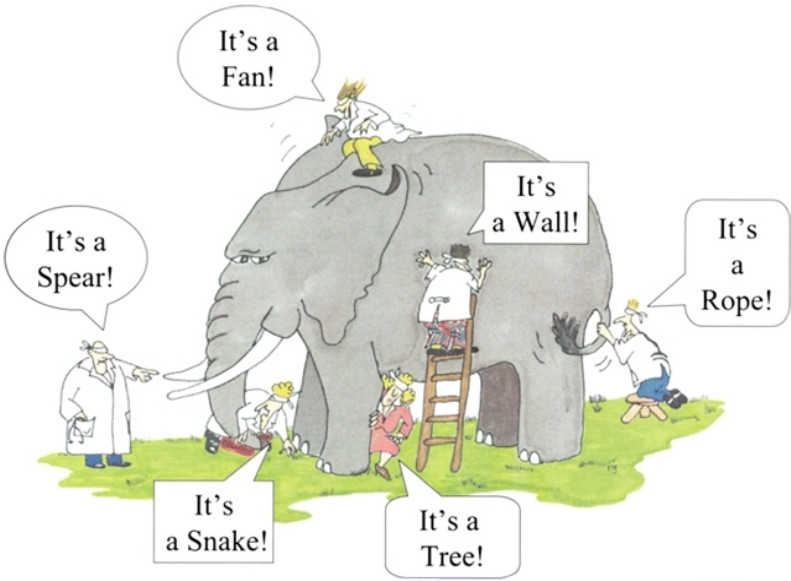
\includegraphics[width=8cm]{introduccion/elephant.jpg}\hspace{\fill}

